\documentclass[main.tex]{subfiles}
\begin{document}
\chapter{Resultate} 

\section{Performance}
Die Tests ergaben eine aufschlussreiche Datenmenge in Hinblick auf die Performance. Dabei sind nicht allein der Durchsatz und die Latenzzeit wichtige Indikatoren. Es gilt ebenfalls zu analysieren, wie die Ressourcen auf der PaaS genutzt wurden. Dabei werden die Daten miteinander verglichen und mögliche Ursachen für die Performance aufgezeigt. 

% Wie ändert sich das Antwortzeitverhalten in Abhängigkeit von der Last?
% Kann mit dem System auch unter hoher Last noch akzeptabel gearbeitet werden?
% Zeigt das System undefiniertes Verhalten (z. B. Absturz)?
% Geht das System nach Rückgang der Überlast wieder in den normalen Bereich zurück?


\subsection{Durchsatz nach Anfragen}
Wie in der Abbildung \ref{figure:throughputSzen} ersichtlich wird, haben alle OSRE verschiedene Durchsatzrates erzeugt.

\subsubsection{Szenario 1 und 2}
Der höchste Durchsatz gelang mit Apache PDFBox. Der maximale Durchsatz in der Testreihe betrug 151 Anfragen pro Sekunde. Dies wurde beim Szenario 1 mit der Rate von 50 virtuellen Usern erreicht.  Apache PDFBox hat bei Durchsatz und Verarbeitungsgeschwindigkeit in den ersten beiden Szenarien die höchste Rate im Vergleich zu iText und JasperReports erreicht. 
Der Durchsatz lag beim ersten und zweiten Szenario mit Apache PDFBox bei über 100 Anfragen pro Sekunde, ausser bei den Szenarien 1b und 2b, bei denen die zu verarbeitenden Daten verdreifacht wurden. 
iText zeigt ähnliche Ergebnisse, dies mal mit dem Maximal Durchsatz von 60 Anfragen pro Sekunde im Szenario 2 mit ebenfalls 50 virtuellen Usern. Der Durchsatz von iText und Apache PDFBox schwankt stark. Ein Vergleich vom besten Ergebnis (Szenario 1c) zum schwächsten (Szenario 1b) mit Apache PDFBox zeigt eine Verschlechterung des Durchsatzes von bis zu 60.9\%. Auch bei iText ist eine Verminderung des Durchsatzes festzustellen, die  bis zu 83\% betrug. Hingegen blieb der Durchsatz bei JasperReports vergleichsweise konstant. JasperReports zeigt bei allen Szenarien einen Durchsatz zwischen 11 und und 17 Anfragen pro Sekunde und eine robustere, jedoch langsame Implementierung des Service.\newline 
\subsubsection{Szenario 3}
Das dritte Szenario zeigt eine rapide Abnahme der Durchsätze. Alle drei OSREs bringen den Durchsatz nicht über 15 Anfragen pro Sekunde. Das bedeutet, dass im besten Fall das Szenario 3 von JasperReports 52'200 mal in einer Stunde verarbeitet werden kann. iText würde etwa 34'200 PDF in der gleichen Zeit generieren und Apache PDFBox gerade mal 18'360 PDFs liefern. 
Apache PDFBox hat in diesem Szenario die langsamste Verarbeitung mit 1.8 Anfragen pro Sekunde, knapp gefolgt von iText mit 3.1 Anfragen pro Sekunde. 

\begin{figure}[!ht]
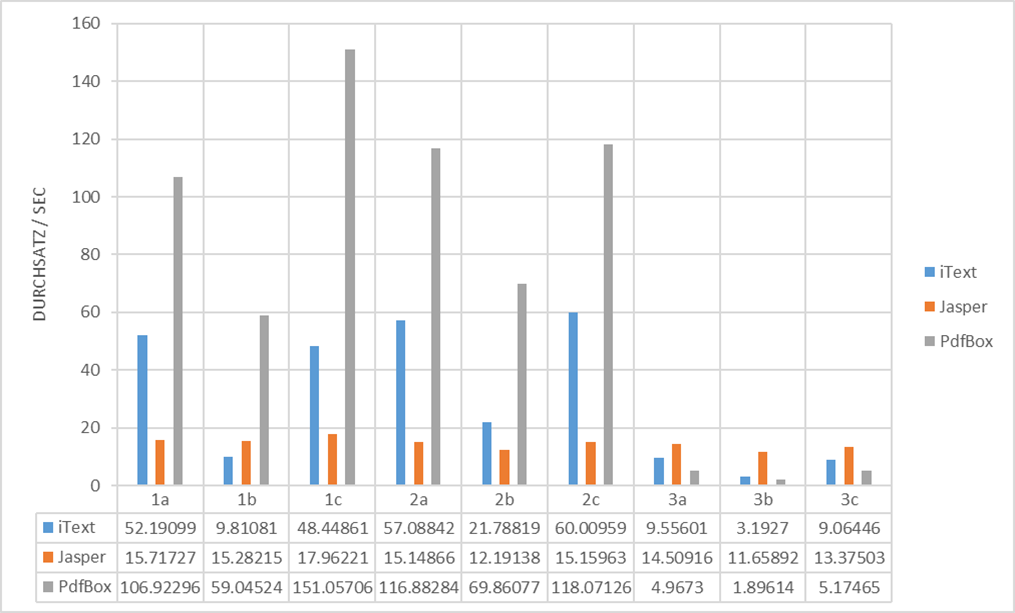
\includegraphics[width=\textwidth]{mainpart/4_analyse_img/VglDurchSzen.png}
 \caption{Vergleich - Durchsatz nach Szenario}
 \label{figure:throughputSzen}
\end{figure}

\subsection{Durchsatz nach Bytes}
Die Abbildung \ref{figure:throughputBytesAll} zeigt, dass der Durchsatz in Bytes über die Testdauer hinweg nicht einbricht. Der Durchsatz nach Bytes scheint nur bei JasperReports tief zu bleiben. Der Durchsatz nach Bytes scheint auch bei Apache PDFBox und iText beim Szenario 3 zu steigen,  wobei der Durchsatz der Antworten nachlässt. Analysiert man die Grösse der Antworten, wird auch klar warum. 
\begin{figure}[!h]
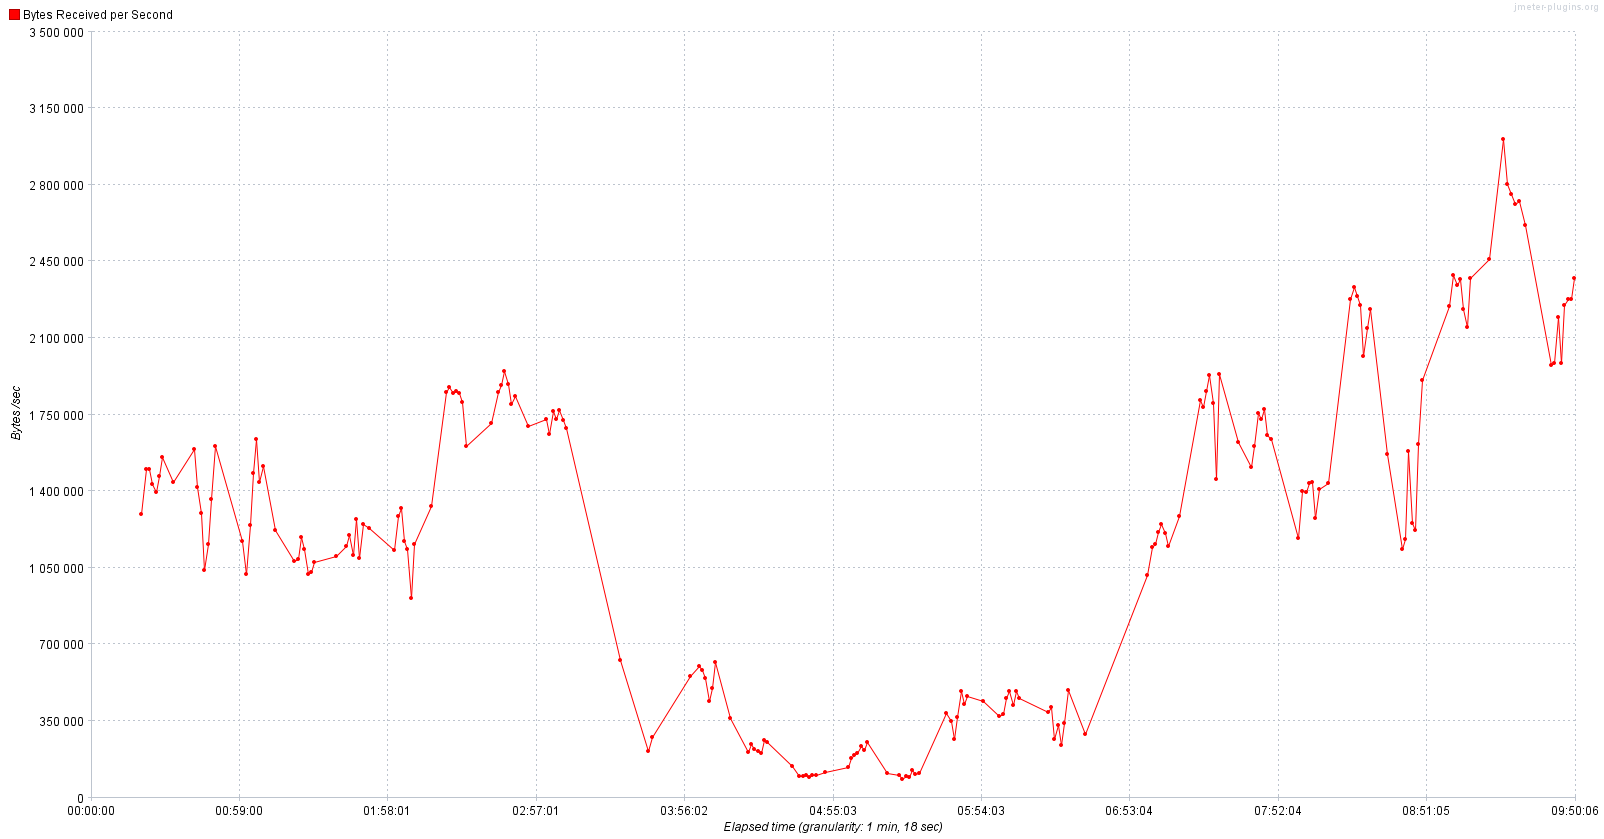
\includegraphics[width=\textwidth]{mainpart/4_analyse_img/ThroughputOverTimeAll.png}
 \caption{Durchsatz in Bytes}
 \label{figure:throughputBytesAll}
\end{figure}


% Diskussion verschoben werden
JasperReports generiert im Vergleich zu den anderen OSREs weitaus kleinere PDFs. Die Kontaktliste, eine Liste mit Kontaktdaten und einem Gender-Symbol, die im Szenario 3 generiert wird, verarbeitet JasperReports besser als die anderen OSREs. Es scheint, als ob die Bilder referenziert und komprimiert würden. Dies ist mithilfe der vorkompilierten Templates möglich. Das mit JasperReports generierte PDF ist etwa 46KB gross, das mit Apache PDF-Box generierte PDF ist etwa 730KB gross. Etwas besser ist die Komprimierung bei iText, mit dem das PDF etwa 350 KB gross wird. Dies bedeutet zwar, dass der Durchsatz nicht vergrössert wurde, doch die generierten Files nutzten dennoch die Bandbreite des verfügbaren Netzwerkes. Wie gross die Bandbreite eines Webservice ist und welche Netzwerkverbindung den Engpass darstellte, konnte nicht festgestellt werden. 


\subsection{Latency}
%Min / Max Average --> Vergleichen mit anderen Projekten wer hat die kürzeste Latenz wer die längste

Die Latenzzeit, die in der Abbildung \ref{figure:latencyTestcycle} dargestellt wird, ist die Zeit, die der Service gebraucht hat, um die Anfrage zu bearbeiten, samt Netzwerkzeit. 

% Diskussion
Diese Grafik korreliert klar mit der Analyse der Durchsätze. Der Durchsatz steigt umgekehrt proportional zur gemessenen Latenzzeit.

\begin{figure}[!ht]
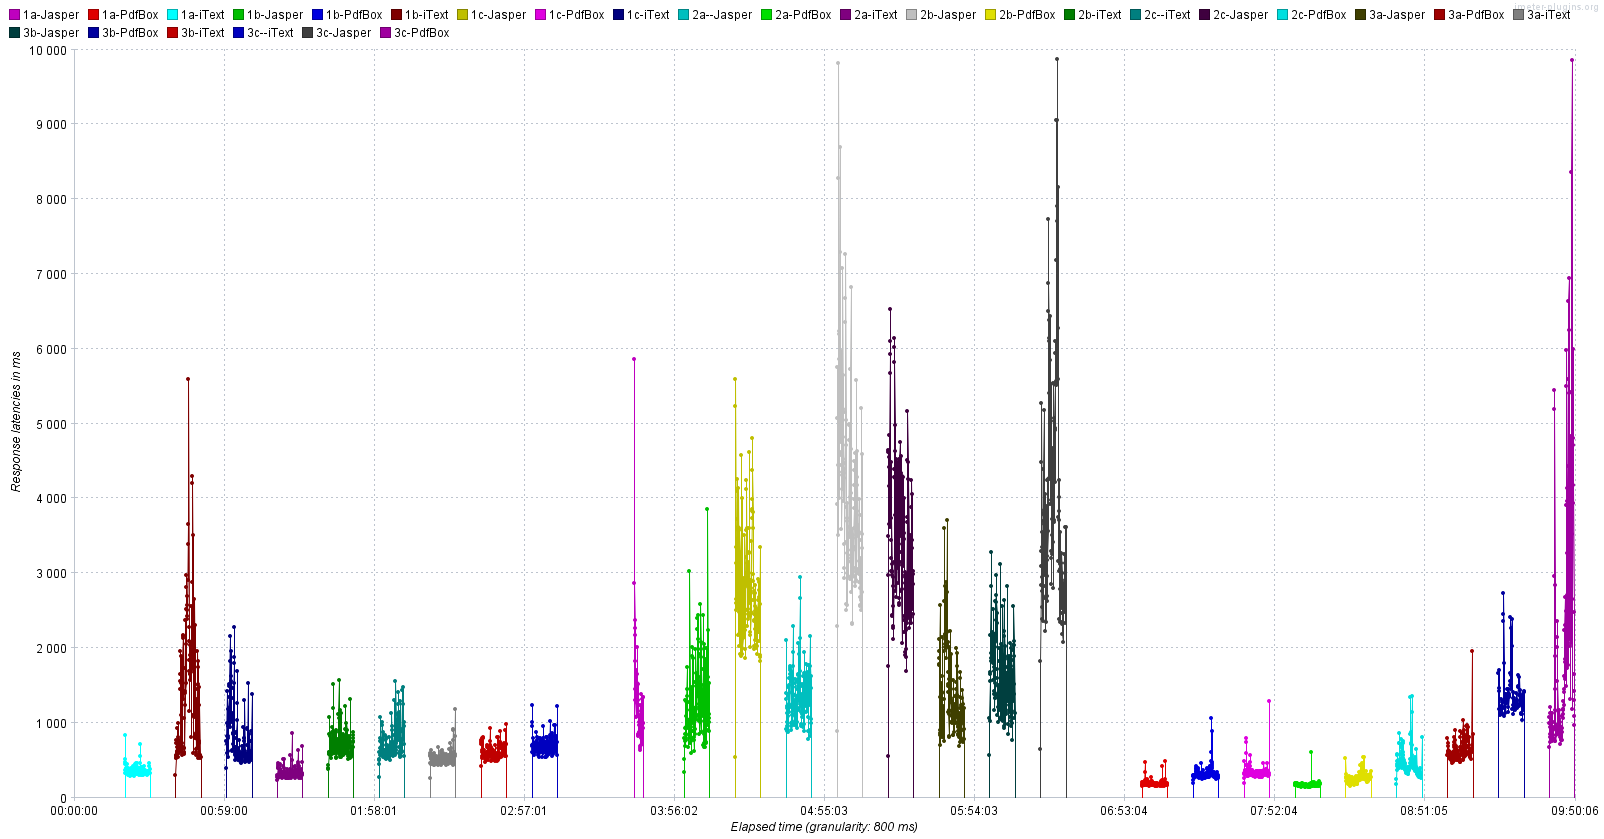
\includegraphics[width=\textwidth]{mainpart/4_analyse_img/ResponseLatenciesOverTime.png}
 \caption{Latenzzeit im Testzyklus}
 \label{figure:latencyTestcycle}
\end{figure}




Auch hier kommen iText und Apache PDFBox bei den meisten Szenarien mit weniger als einer Sekunde aus. Doch es sind auch Ausnahmen festzustellen, wie beim Szenario 1b bei iText und im Szenario 3 bei Apache PDFBox. Diese Latenzzeiten sind keine Aussage zur Netzwerklatenz, die reine Zeit, die verbraucht wird, bis eine Nachricht vom Sender zum Empfänger übermittelt wurde. Diese Zeit gibt die reine Antwortzeit des Service wieder. Auch bei Abbildung \ref{figure:latencySzenario} vergrössert sich die Latenz wegen der Verarbeitungszeit während des Szenarios 3. JasperReports zeigt dabei eine überdurchschnittliche Latenzzeit während der ersten beiden Szenarien.
% Diskussion
%% Der Serviec ist in den USA ist die Netzwerklatenz so gross um Hunderte oder sogar tausende von Antworten zu stoppen ? 

\begin{figure}[!ht]
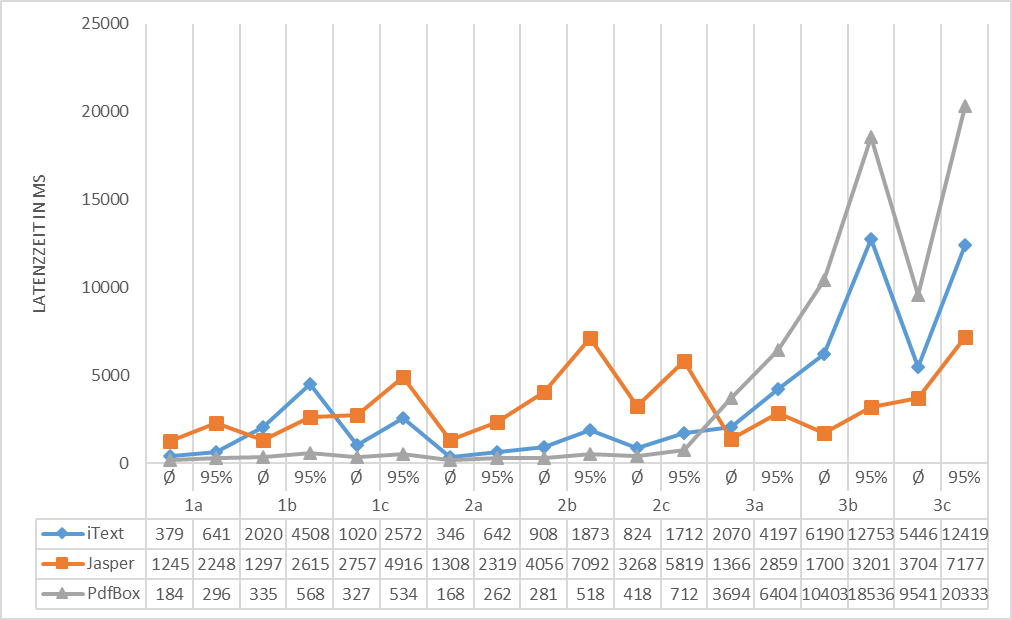
\includegraphics[width=\textwidth]{mainpart/4_analyse_img/LatenzzeitSzen.png}
 \caption{Latenzzeit nach Szenario und OSRE}
 \label{figure:latencySzenario}
\end{figure}

\subsection{Verfügbarkeit}

Der Service soll auch über die Zeit hinweg möglichst verfügbar bleiben. Dies ist ebenfalls ein wichtiger Performance-Indikator. Während der Tests hat keiner der Services über den Testlauf von rund drei Stunden einen Absturz gehabt oder ist unerreichbar gewesen. Die Prototypen waren im Verlauf der Tests meist aktiv geblieben, was aber nicht heisst, dass ein User diese auch als verfügbar empfunden hätte. Hätte man diese Prototypen in einer Produktionsumgebung eingesetzt, wäre der User wohl des Öfteren mit längeren Wartezeiten konfrontiert gewesen. 
Die Latenzzeiten, die im vorhergehenden Kapitel erwähnt wurden, wären auch hier ein Thema. In der Abbildung \ref{figure:latencySLA2000} wird ersichtlich, wie viel Prozent der Anfragen an die entsprechenden Services länger gedauert hätten als 2 Sekunden.

\begin{figure}[!ht]
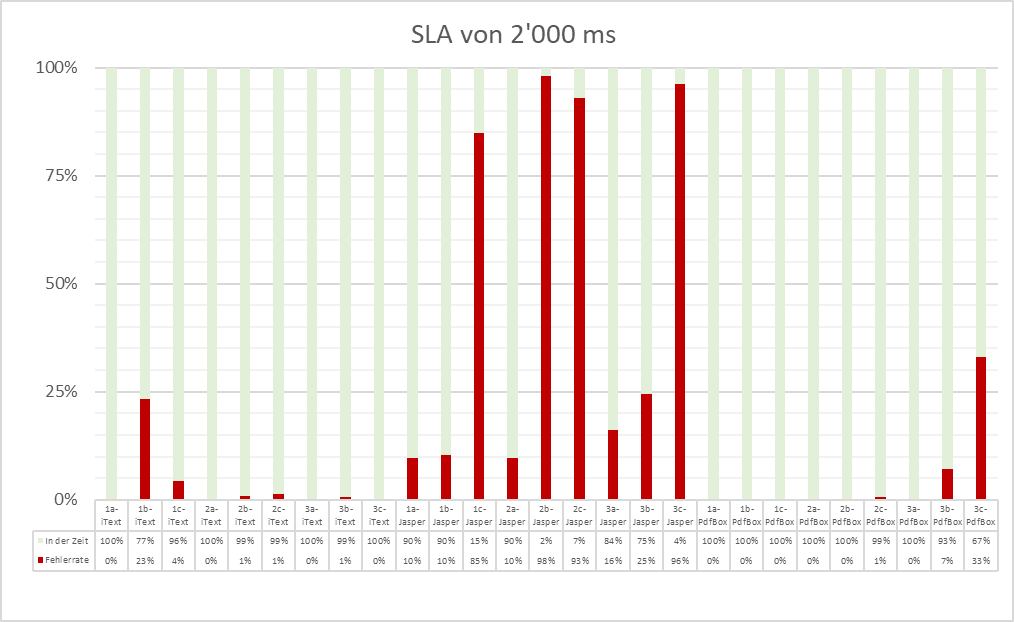
\includegraphics[width=\textwidth]{mainpart/4_analyse_img/latencySLA2000.png}
 \caption{Fehlerrate nach Latenzzeit über 2000ms}
 \label{figure:latencySLA2000}
\end{figure}


% Diskussion  oder Grundlagen?
Nach Miller \cite[Seite~270]{miller_1968} sind Verzögerungen erst dann ein Problem, wenn diese mit dem Fluss der spezifischen Arbeit zusammenkommen. Ein Betriebssystem muss immer in weniger als 0.1 Sekunden antworten, damit es den Arbeitsfluss nicht behindert. Auch hat ein Schreibprogramm in weniger als einer Sekunde zu reagieren, auch wenn Graphiken verarbeitet werden, damit der User in seinem kreativen Prozess nicht behindert wird. Weiter sind die Zeitspannen von 2 bis 4 Sekunden ebenfalls eine wichtige Grösse. Bei komplexen Arbeiten, bei denen der User sich Informationen merken muss, ist es wichtig, diese Antwortzeit so gering wie möglich zu halten.

In der Abbildung \ref{figure:latencySLA2000} wird gezeigt, dass sich besonders JasperReports für eine Online-Applikation nicht wirklich eignete. Vier von neun Szenarien benötigen meist mehr als 2 Sekunden, um eine initiale Antwort zu senden. Die Latenzzeit beträgt bei mehr als 85\% der Antworten mehr als 2 Sekunden. Dies wäre für den Online-Benutzer zu lange, wenn diese Daten für seinen Arbeitsprozess nötig wären.

JasperReports liefert 99\% der Antworten innerhalb von 10 Sekunden, was für eine Batchverarbeitung akzeptabel wäre. Dennoch haben auch iText und Apache PDFBox bei einer SLA von zwei Sekunden in einigen Fällen Schwierigkeiten. iText hat bei der Verarbeitung des Szenarios 1b eine Verfügbarkeit von 77\% erreicht, was zu tief ist für eine Online-Verarbeitung. Bei den übrigen Szenarien, mit der kleinen Ausnahme des Szenarios 1c, das bei 96\% angelangt ist, konnte bei 99\% eine Antwortzeit von unter zwei Sekunden erreicht werden.

Apache PDFBox zeigt hingegen wieder, dass die Verarbeitung der Reports im Szenario 3b und 3c oft eine Geschwindigkeit erreicht, die der User nicht mehr als angenehm oder akzeptabel empfinden würde.








\section{Resourcen}

Welche Auswirkung die Test auf dem Webservern haben wird in den folgenden Kapitel behandelt. 

\subsection{Arbeitsspeicher}

Aus den Performance-Messungen konnte der Verbrauch auf der PaaS geloggt werden und ist in der Abbildung \ref{figure:memorytestlauf} zu sehen. Die Memoryauslastung steigt bei der Ausführung der Performancetests und sinkt bei der Ausführung des GC oder einem Neustart des Webservers (Dynos). Die Dynos sind als Standard-X2 definiert, was bedeutet, dass die maximale Auslastung auf den Memory RSS auf 1024MB beschränkt ist. Dies bedeutet, dass die Auslastung auf dem Memory begrenzt ist und jede weitere Verarbeitung auf den SWAP ausgelagert wird. Die Abbildung \ref{figure:memorytestlauf} zeigt diese Phänomene. iText nutzte nur wenig SWAP und konnte in den Performancetests mit RSS Memory meist alle Anfragen bearbeiten. Ein Teil der Anfragen wurde dennoch im Szenario 3 im SWAP ausgelagert. Nach einem Restart des Webservices wurde JasperReports genutzt. Diese ORSE nutzte bereits das verfügbare Memory im ersten Szenario. Das Memory auf dem SWAP konnte über alle Szenarien hinweg nicht freigegeben werden, was zu einem Aufblasen des Memoryverbrauchs führte. JasperReports erreichte im Testlauf einen totalen Memoryverbrauch von 1389.32MB. Apache PDFBox erreichte im Testlauf die Memory-Quota kaum.




\begin{figure}[!ht]
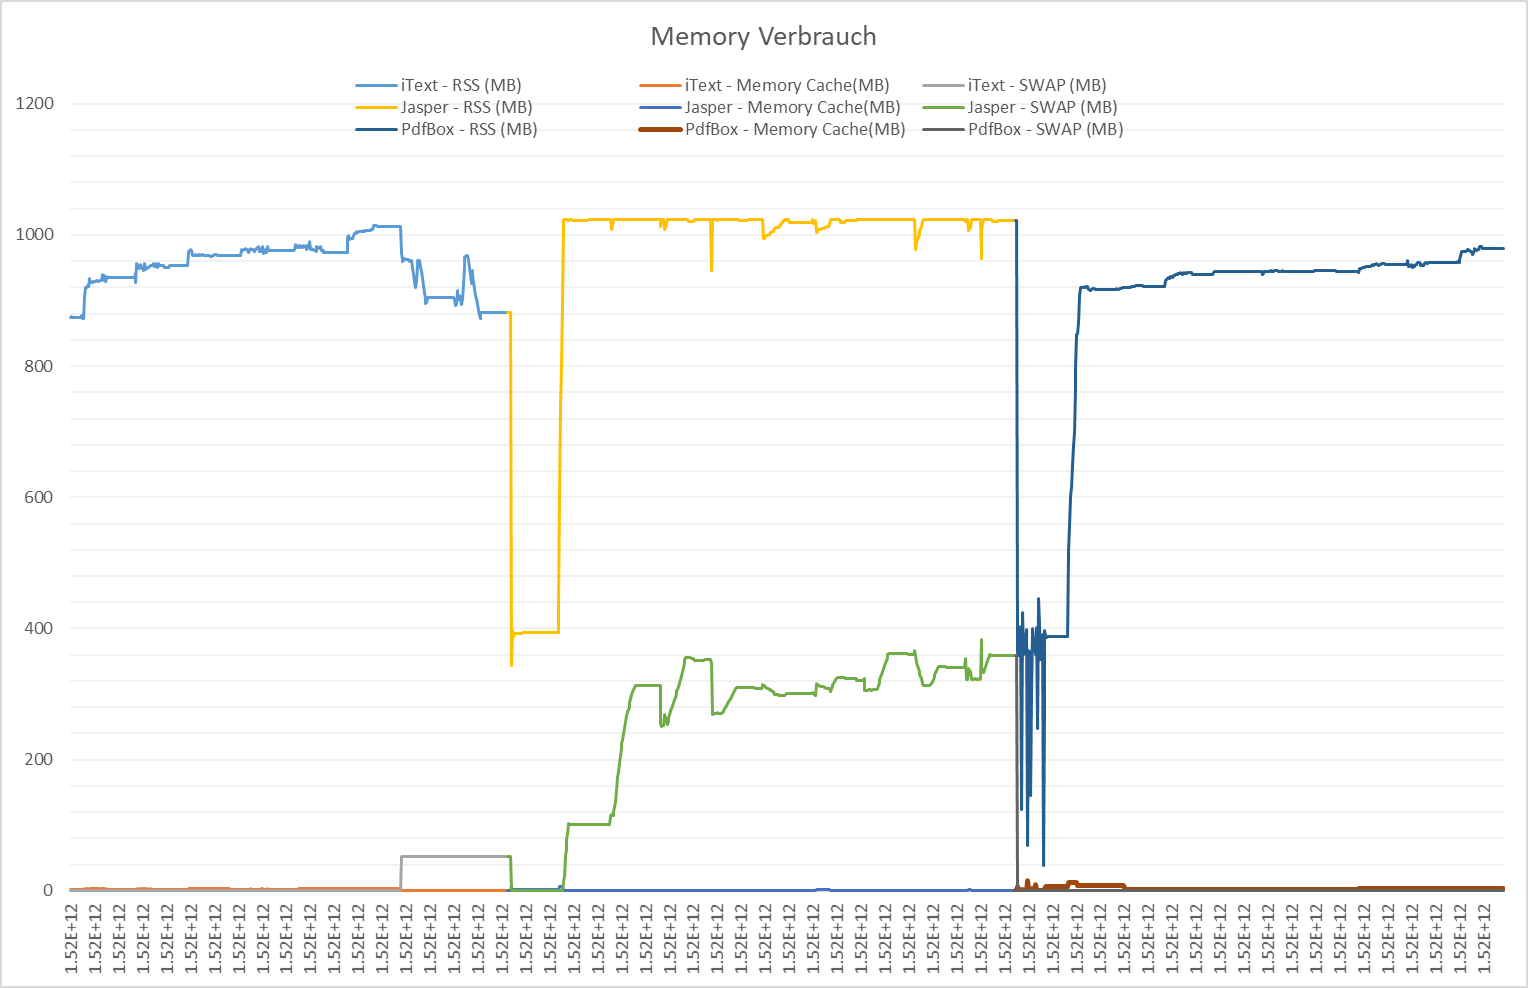
\includegraphics[width=\textwidth]{mainpart/4_analyse_img/MemoryVerbrauch.png}
 \caption{Memoryverbrauch Testlauf}
 \label{figure:memorytestlauf}
\end{figure}



\subsection{Prozessor Last}

Der Verbrauch des \acrshort{cpu} ist eine etwas schwierige Messgrösse. Die \acrlong{paas} hat diese Daten mit der Stichprobengrösse von einer Minute in die Logs geschrieben.

Dabei ist natürlich zu erkennen, dass sich im Textzyklus von iText  die Auslastung je nach Szenario sehr stark unterscheidet. Z.B. sind während des zweiten Szenarios durchschnittlich zwischen vier und sieben Prozessoren im Status 'Ready' pendent gewesen. Hingegen sind im dritten Szenario fast immer alle Prozessoren in Ausführung gewesen, das bedeutet eine fast optimale Auslastung des CPUs mit wenigen wartenden Prozessen. Diese sind wohl so entstanden, da die Prozesse im dritten Szenario langläufiger waren und somit wenig neue Anfragen verarbeitet wurden.

JasperReports hat den CPU eher gefordert und hat über den ganzen Zeitraum viele Prozesse gebraucht. Wie intensiv die Verarbeitung von JasperReports im Vergleich zu den anderen OSREs ist, wird hier klar hervorgehoben



Apache PDFBox ist hier als sehr sparsam zu erkennen. Es wurden maximal fünf Prozesse ausgelagert. 
\begin{figure}[!hb]
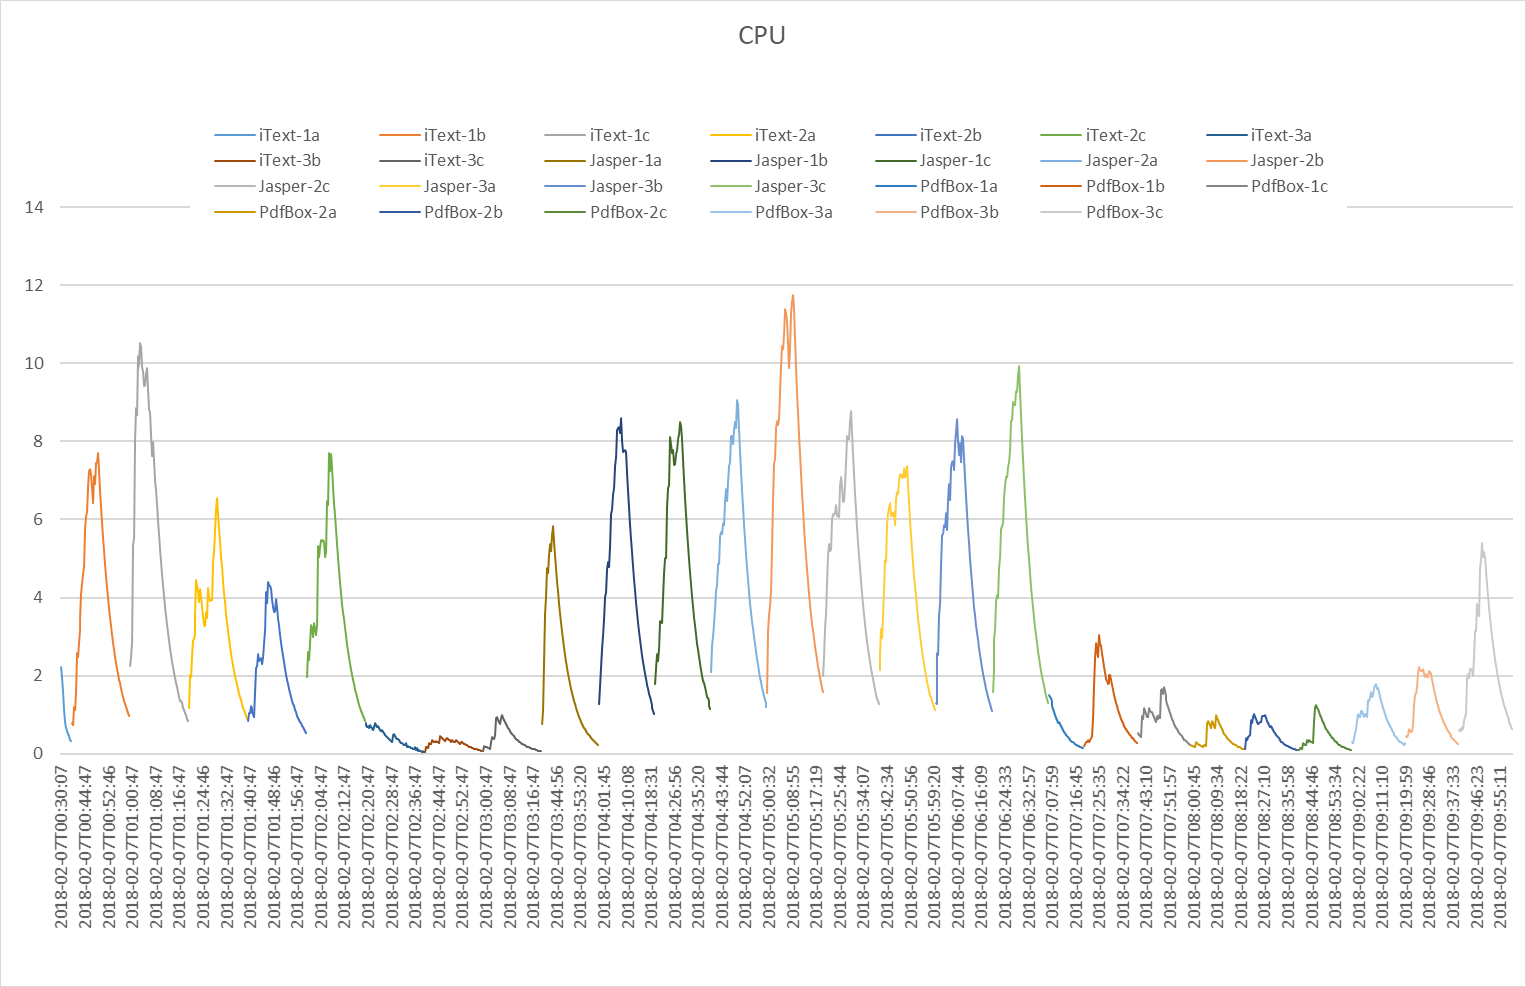
\includegraphics[width=\textwidth]{mainpart/4_analyse_img/CPUVergleich.png}
 \caption{Vergleich - Durchsatz nach Szenario}
 \label{figure:cpuVergleich}
\end{figure}




\section{Reporting Engines - Verhalten}

Die OSREs haben sich während des Tests in Bezug auf die Lastveränderung verschieden verhalten. In diesem Kapitel sollen die Veränderungen von Requestgrössen und die Zunahme von virtuellen Usern (\acrshort{vu}) weiter aufgezeigt werden.


\subsection{Requestgrösse}
Im Vergleich zu den Szenarien 1a, 2a und 3a wurden bei den Szenarien 1b, 2b und 3b die Datensätze für die Verarbeitung verdreifacht. Wie den Abbildungen \ref{figure:vglABRequ} entnommen werden kann, hat dies dazu geführt, dass sich alle Antwortzeiten und Durchsätze verschlechtert haben

\begin{figure}[!hb]
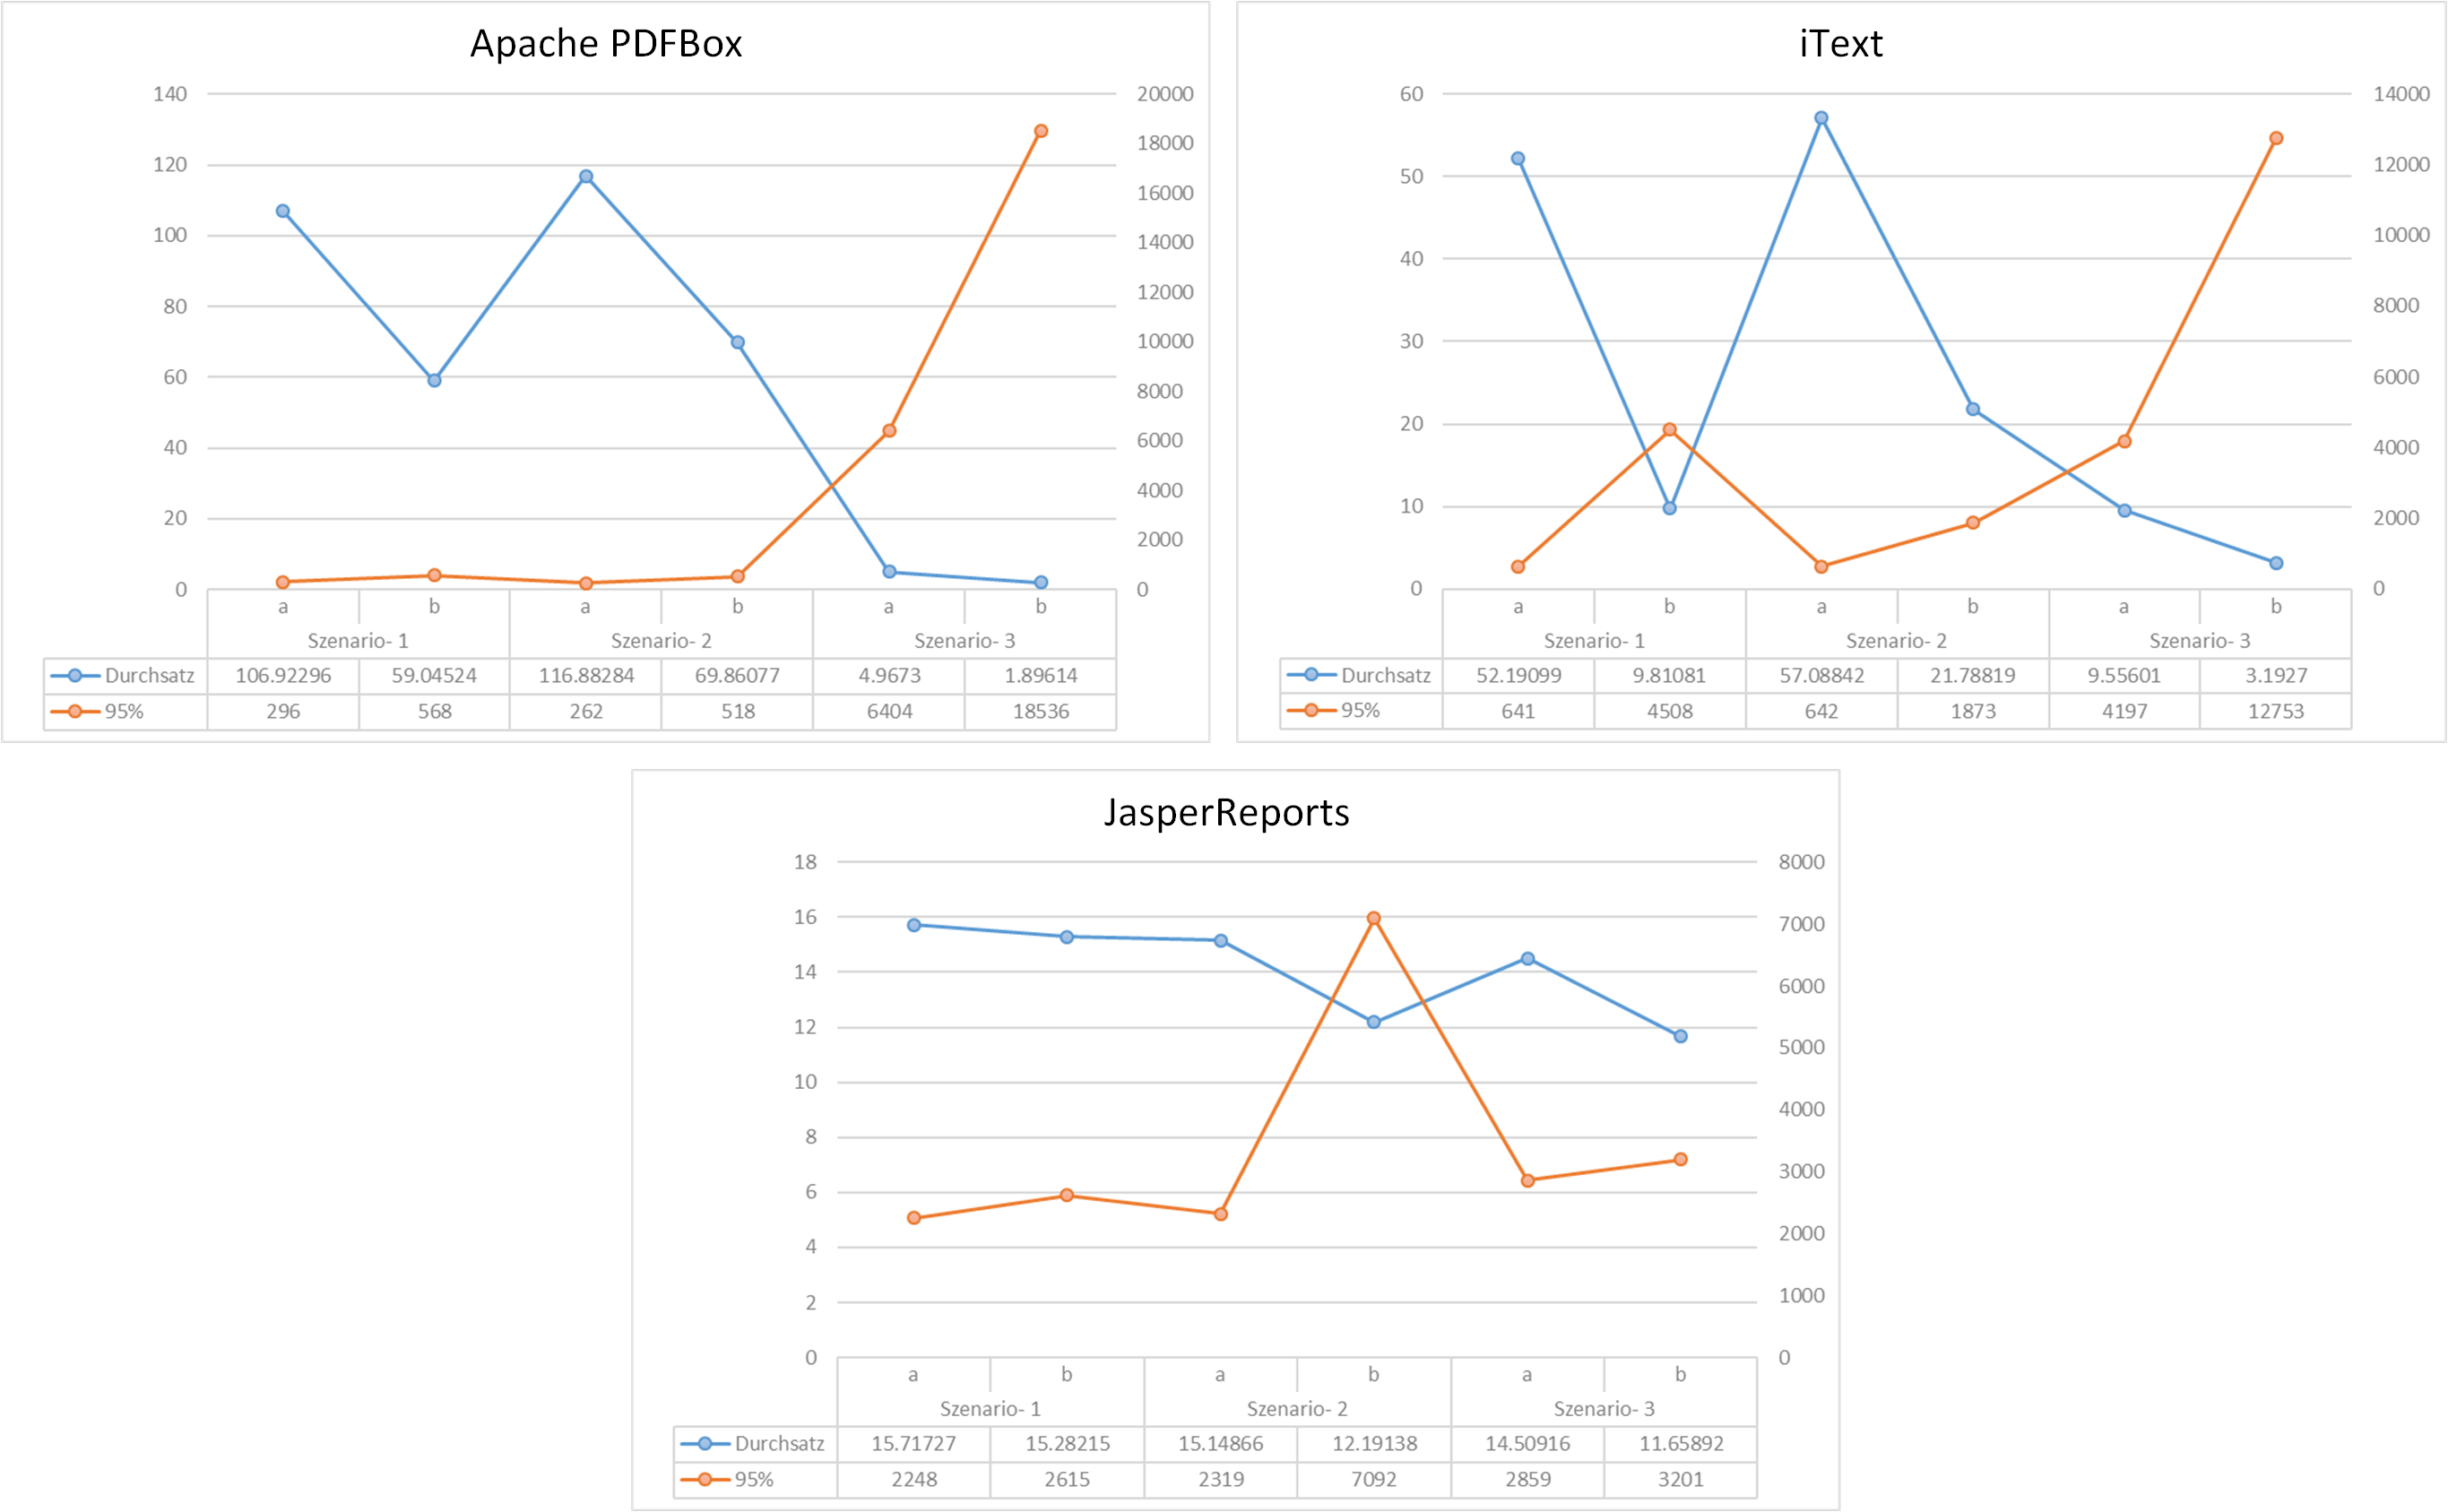
\includegraphics[width=\textwidth]{mainpart/4_analyse_img/ABAuswertung.png}
 \caption{Vergleich Baseline mit grösserer Datenmengen}
 \label{figure:vglABRequ}
\end{figure}

OSRE, iText und Apache PDFBox haben sich in der gleichen Art und Weise verschlechtert. iText verzeichnet hier Durchsatzeinbrüche. Die ersten zwei Szenarien fallen je von zwischen 50 und 60 auf fast 10 und 21 Anfragen pro Sekunde.

Hier sei noch einmal hervorgehoben, dass diese Daten aufgrund eines Testlaufs ermittelt wurden. Es kann in jedem Testlauf das gleiche Phänomen beobachtet werden, dennoch sind diese Daten nicht stellvertretend oder absolut zu betrachten. Grössere Ausreisser wurden in anderen Testläufen aufgezeichnet.





\subsection{Virtuelle User}
Die Prototypen wurden von den initialen 20 \acrshort{vu} im Szenario 'a' weiter gefordert, als 30 weitere \acrshort{vu}s hinzugefügt wurden, um eine erhöhte Nutzerinteraktion zu simulieren. Wie die s dabei reagiert haben, kann in der Abbildung \ref{figure:vglACVU} gesehen werden. In den Abbildungen werden die Veränderungen des Durchsatzes mit dem 95 Perzentil der Antwortzeit verglichen. Dabei ist nur massgebend, wie sich die \acrshort{osre}s im Durchschnitt verhalten.

\begin{figure}[!ht]
\includegraphics[width=\textwidth]{mainpart/4_analyse_img/ACAuswertung.png}
 \caption{Vergleich Baseline mit mehr virtuellen Usern}
 \label{figure:vglACVU}
\end{figure}

Einige der interessanten Erkenntnisse in diesem Zusammenhang können bei Apache PDF-Box entdeckt werden. Obwohl die Nutzerlast steigt, steigt auch der Durchsatz im Szenario 1 von 106 auf 151 Anfragen pro Sekunde. Die Antwortzeit verdoppelt sich aber dabei. Ähnliches ist auch im zweiten Szenario zu beobachten. Beim Kreuzvergleich mit der Zunahme der zu verarbeitenden Daten (Abbildung \ref{figure:vglABRequ}) sieht man klar, dass diese im Durchsatz einen deutlichen Einbruch erleben, aber die Antwortzeit gleich bleibt. Apache PDFBox hat klar Mühe mit dem Szenario 3. Die Antwortzeit verdreifacht sich dabei, wobei der Durchsatz gleich bleibt.


iText scheint in der Implementation der ersten zwei Szenarien ein ähnliches Verhalten unter Last zu erzeugen. Die Antwortzeit wird im ersten Szenario viermal langsamer, im Szenario 2 dreimal langsamer. Auch iText schafft es, seinen Durchsatz zu verbessern, und zwar werden drei Antworten mehr pro Sekunde verarbeitet. Szenario 3 hat ähnliche Probleme wie Apache PDFBox. Die Antwortzeiten verdreifachen sich und der Durchsatz bleibt auch bei iText etwa konstant.

JasperReports verschlechtert sich in allen Antwortzeiten, aber nicht ganz so extrem wie iText und Apache PDFBox. In allen Szenarien verschlechtern sich die Antwortzeiten. Bei allen Szenarien wurde JasperReports etwa doppelt so langsam. Was den Durchsatz anbelangt, blieb dieser fast konstant, im Szenario 1 wurde dieser ebenfalls etwas höher (2 Anfragen pro Sekunde mehr).




\section{Ursachenanalyse}


Im Szenario 3 konnte man den Rückgang von iText und Apache PDFBox erkennen. Es lässt sich anhand der Ergebnisse der verschiedenen Metriken die Schlussfolgerung ziehen, dass der Durchsatz nicht durch eine Netzwerk- oder Infrastrukturstörung herbeigeführt wurde. Es ist fraglich, ob diese schlechte Performance einen Zusammenhang mit anderen nicht beinflussbaren Einflussfaktoren hat. Dennoch zeigt sich einerseits, dass die Implementierung im Zusammenhang mit dem Szenario 3 zur Generierung von vergleichsweise grossen PDFs führte. Andererseits sind Aufbau und Layout bei iText und Apache PDFBox mit mehr Rechenleistung verbunden. Apache PDFBox zeigt bei der Last auf dem PaaS-Provider eine höhere Last bei der Ausführung des Szenarios 3. iText wiederum zeigt keine Zunahme, sondern sogar einen Rückgang der CPU-Last.

Bei der Analyse mittels Java visual VM wurde ersichtlich, dass bei der Ausführung von JasperReports viele Objekte angelegt werden, die im Zusammenhang mit den Jasper-Templates stehen. Jedes Feld wird dabei ausgelesen und als Ressource gehalten.


\end{document}